%%%%%%%%%%%%%%%%%%%%%%% file template.tex %%%%%%%%%%%%%%%%%%%%%%%%%
%
% This is a general template file for the LaTeX package SVJour3
% for Springer journals.          Springer Heidelberg 2010/09/16
%
% Copy it to a new file with a new name and use it as the basis
% for your article. Delete % signs as needed.
%
% This template includes a few options for different layouts and
% content for various journals. Please consult a previous issue of
% your journal as needed.
%
%%%%%%%%%%%%%%%%%%%%%%%%%%%%%%%%%%%%%%%%%%%%%%%%%%%%%%%%%%%%%%%%%%%
%
% First comes an example EPS file -- just ignore it and
% proceed on the \documentclass line
% your LaTeX will extract the file if required
\begin{filecontents*}{example.eps}
%!PS-Adobe-3.0 EPSF-3.0
%%BoundingBox: 19 19 221 221
%%CreationDate: Mon Sep 29 1997
%%Creator: programmed by hand (JK)
%%EndComments
gsave
newpath
	20 20 moveto
	20 220 lineto
	220 220 lineto
	220 20 lineto
closepath
2 setlinewidth
gsave
	.4 setgray fill
grestore
stroke
grestore
\end{filecontents*}
%
\RequirePackage{fix-cm}
%
%\documentclass{svjour3}                     % onecolumn (standard format)
\documentclass[smallcondensed]{svjour3}     % onecolumn (ditto)
%\documentclass[smallextended]{svjour3}       % onecolumn (second format)
%\documentclass[twocolumn]{svjour3}          % twocolumn
%
\smartqed  % flush right qed marks, e.g. at end of proof
%
\usepackage{algorithmic}
\usepackage{amsmath,amssymb,amsfonts}
\usepackage{enumerate}
\usepackage{wrapfig}
\usepackage{graphicx}
\usepackage{appendix}
\usepackage{graphicx}
\usepackage{amsmath}
\usepackage{caption}
\usepackage{subfigure}
\usepackage{makecell}
\usepackage{multirow}
\usepackage{booktabs}
\usepackage{threeparttable}
\usepackage{geometry}
\usepackage{float}
\usepackage{indentfirst}
\usepackage[colorlinks,
linkcolor=blue,
anchorcolor=black,
citecolor=blue]{hyperref}
\geometry{top=2.5cm,bottom=2.5cm}
%
% \usepackage{mathptmx}      % use Times fonts if available on your TeX system
%
% insert here the call for the packages your document requires
%\usepackage{latexsym}
% etc.
%
% please place your own definitions here and don't use \def but
% \newcommand{}{}
%
% Insert the name of "your journal" with
% \journalname{myjournal}
%
\begin{document}
	
\title{Research on Human Posture Transfer Based on EDHR-GAN%\thanks{Grants or other notes
		%about the article that should go on the front page should be
		%placed here. General acknowledgments should be placed at the end of the article.}
}
	%\subtitle{Do you have a subtitle?\\ If so, write it here}
	
	%\titlerunning{Short form of title}        % if too long for running head
	
	\author{xx* $^{1}$ \and xx $^{1}$ \and xx*$^{1}$ \and  xx $^{1}$ \and  xx $^{1}$ \and xx $^{1}$ \and xx $^{1}$}
	
	%\authorrunning{Short form of author list} % if too long for running head
	
	\institute{xx* \at
		\email{xx}   
		\\
		\and
		xx \at
		\email{xx \\} 
		\and
		xx* \at
		\email{xx \\} 
		%             \emph{Present address:} of F. Author  %  if needed
		\\
		$^{1}$  Faculty of Robot Science and Engineering, Northeastern University, Shenyang 110819, China 
	}
	
	\date{Received: date / Accepted: date}
	% The correct dates will be entered by the editor
	
	
\maketitle
\begin{abstract}
		
This paper mainly studies the problem of human posture transfer, which is of great significance but also faces many difficulties. In particular, our model allows two different pose images (reference images and target images) to be copied into the same pose. The existing work is mainly to estimate the human body structure through a 2D detection point. This method can not represent the human body's personalized posture well and may have the problem of posture missing. In order to make the generated transfer posture more accurate, not the same as the previous methods, we use a serial SNS network. SNS-1 completes the overall transfer of the reference image pose to the target image pose, and the SNS-2 network fine-tunes the false reference image generated by SNS-1. Through the SNS network, the reference image input by the network can be constrained by the corresponding ground truth, so that the network training is more stable and the generated image is more accurate. In order to keep the image information from being lost, we propose the parallel Encoder-Decoder EDHR-GAN, which can transmit the image information well and generate reasonable images after multiple resolution fusion between different branches. We train on Impersonator (iPER) dataset and do extensive experiments, which show that our method is more effective than other models. 
		\keywords{Generative Adversarial Network \and Posture Transfer \and SNS Network  \and EDHR-GAN}
		% \PACS{PACS code1 \and PACS code2 \and more}
		% \subclass{MSC code1 \and MSC code2 \and more}
		
\end{abstract}
	
\section{Introduction}
\label{intro}
	
As deep learning and computer vision collide, they produce many wonderful results and even overturn our original cognition. Along with the development of the GAN \cite{mirza2014conditional} network, it can "regenerate" the fuzzy classic film in the old film in the aspect of image super-resolution so that the worn image can be restored to the clear, delicate, and pleasing light and shadow; it can enrich the limited data in the aspect of data enhancement, to avoid over-fitting; it can reproduce the true content of precious cultural relics and works of art in image restoration, thereby promoting the development of other research fields. In conclusion, the GAN network has penetrated many research fields and achieved remarkable results. But there are still some areas where there is still much room for improvement, and it is worth further study. Based on this, the research direction selected in this paper is human posture transfer based on the GAN network, which can extend the personal re-identification dataset and apply it to human posture video generation.

Human pose transfer is a challenging task, which involves research hotspots such as human pose recognition, image segmentation, and image restoration. As showed in Figure \ref{image01}, gave a single pose of a person, the goal is to synthesize an arbitrary pose of the person. Through the above description, it is not difficult to find that this task involves more research fields, and these fields are only used as an aid to our work, besides, their research status will also have a great impact on our final results. Although the task faces heavy difficulties, it has great application value in character animation, movie, game making, virtual fitting, and so on. Therefore, we believe that the research of this paper is necessary and significant.

\begin{figure*}
	\centering
	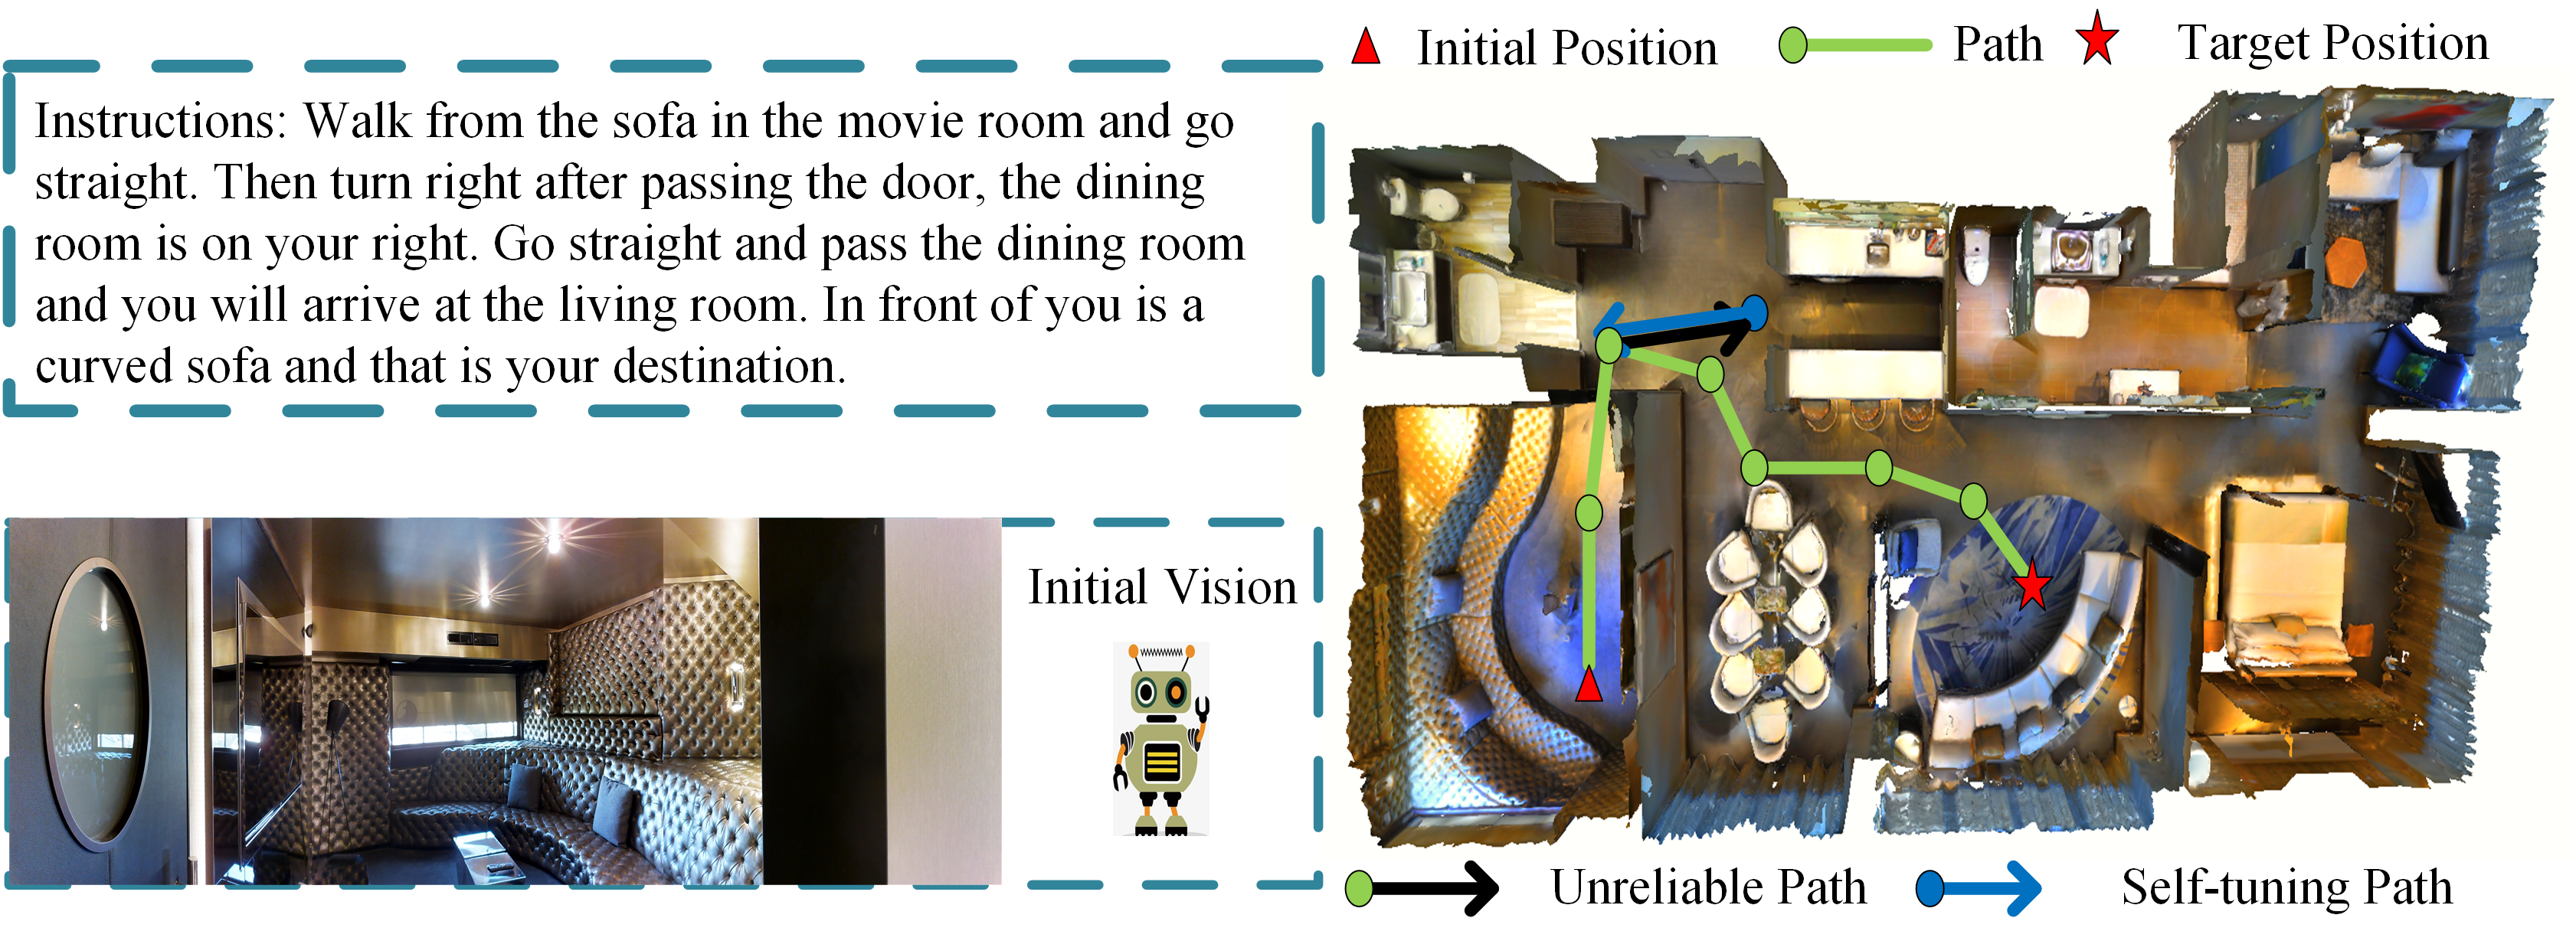
\includegraphics[scale=1]{image01.png}
	\caption{ The first column is a reference image, the second column is a target image, and the third column is a generated false image.}
	\label{image01}
\end{figure*}	

In most of the existing human posture transfer methods ~\cite{chan2019everybody,zhu2019progressive,ma2017pose,ge2018fd}, 2D detection points are used to detect the human posture and directly transfer the 2D posture. The human posture in 3D, especially when large posture changes are carried out, these 2D methods will cause image blurring, posture loss, and other problems that are not in line with reality.
	
To solve these problems, scholars \cite{li2019dense} propose to generate 3D flow from the reference pose and the target pose, and then configure the 3D model to a given pose pair and project them back to the 2D plane to calculate the dense appearance flow of the training. Scholars \cite{liu2019liquid} only use the 3D body network recovery module to decode poses and shapes, and the proposed LWGAN can achieve multiple tasks. Although these methods can alleviate the problems caused by 2D poses, they still produce unreasonable images such as pose distortions.
	 
In order to make the generated pictures have higher quality, this paper proposes a SNS network. The SNS network diagram is shown in Figure \ref{image02}. It can be seen from the figure that the SNS network is mainly divided into three parts: pose extraction network, SNS-1, and SNS-2. Where SNS-1 and SNS-2 belong to two subparts of SNS. According to the SNS network diagram, to complete the human posture transfer task, the specific steps are as follows: First, input the reference image and the target image to the posture extraction network respectively, and then extract the required information to obtain the reference image foreground information, the reference image background information and the target image posture information. Second, the reference image foreground information, the reference image background information, and the target image pose information obtained are fused and conveyed to a generator generating a GAN. The generator contains two parts, one for processing foreground information to complete pose transfer and the other for processing background information to complete background repair. After the generator, the SNS-1 false image is obtained. Third, transfer SNS-1 false image to pose extraction network to obtain SNS-1 image pose information. This completes the SNS-1 phase. Fourth, the SNS-1 image pose information is fused with the reference image foreground information and the reference image background information obtained before, and then transmitted to the generation counter network generator to obtain the SNS-2 false image. At this point, the SNS-2 stage is completed to obtain the desired image of the human posture transfer task. Fifth, send the SNS-1 false image, SNS-2 false image, and target image to the discriminator generating the countermeasure network for true and false discrimination.

\begin{figure*}
	\centering
	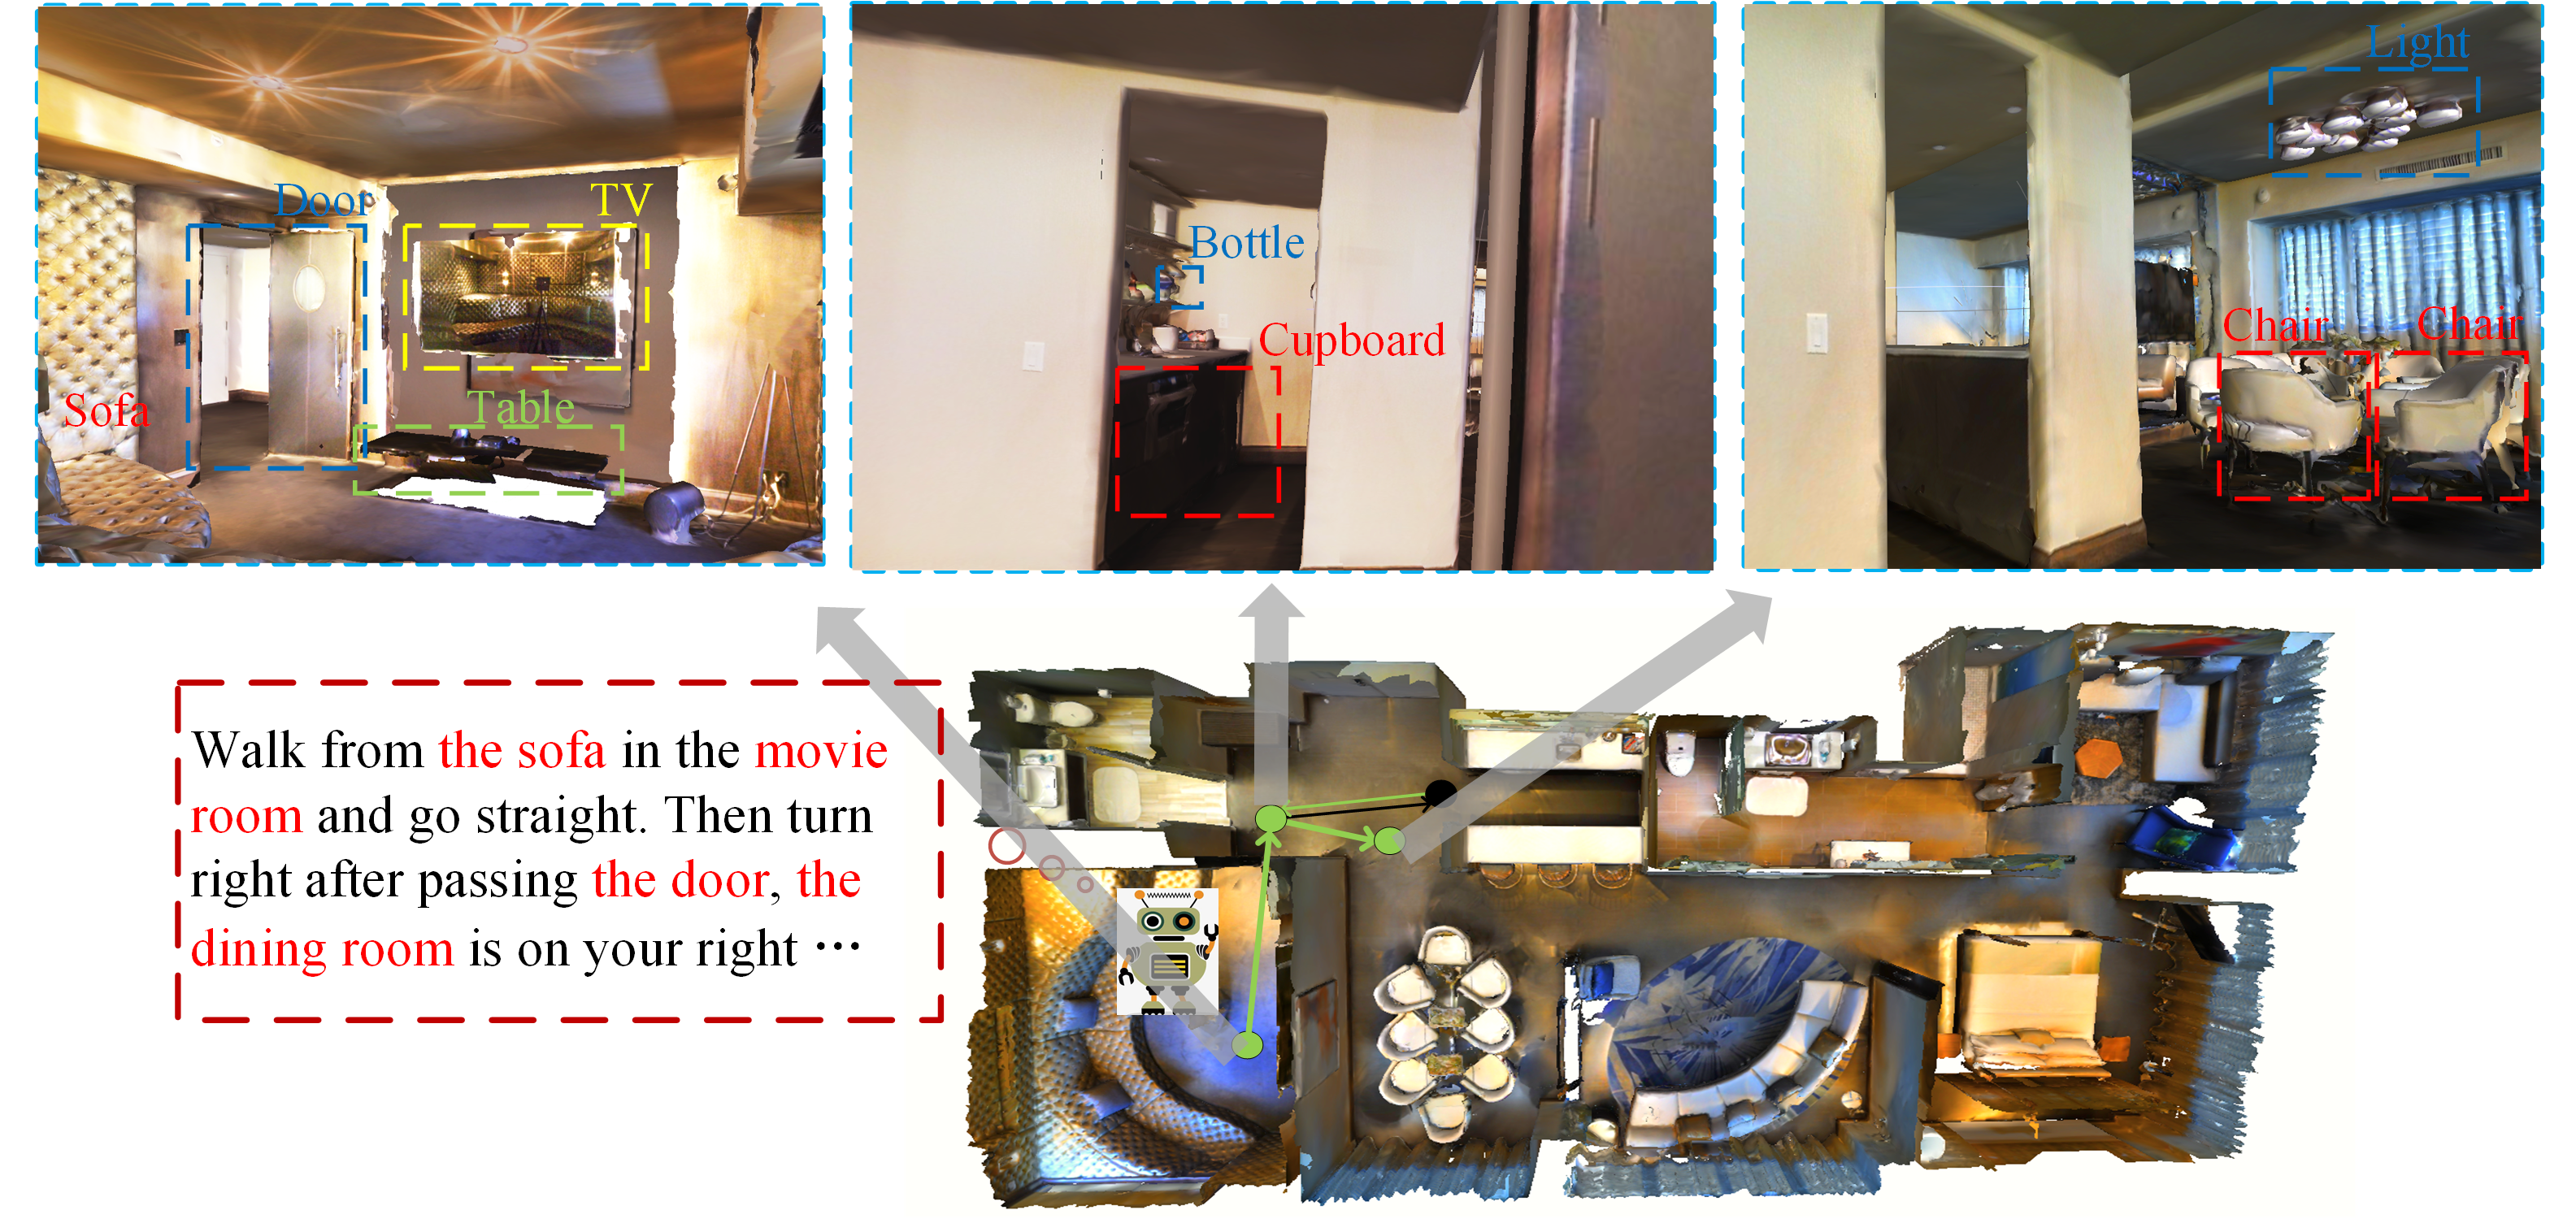
\includegraphics[scale=1.25]{image02.png}
	\caption{ SNS network diagram.}
	\label{image02}
\end{figure*}	

In order to ensure a better generation target pose, in the generator design section, we do not directly adopt the Encoder-Decoder method that is used most of the time. Instead, it combines the idea of end-to-end Encoder-Decoder and the advantage of HRNet network high resolution to build parallel Encoder-Decoder EDHR-GAN. The main network is an Encoder-Decoder, and then parallel branches are added in turn. In the process, the subnets of the same resolution in the network are connected, and the resolution fusion between different branches is carried out multiple times so that the retained information is more accurate.
	
To sum up, the main contributions of this paper are:
\begin{itemize}
		\item[](1) We used 3D pose detection and combined it with EDHR-GAN to enhance the results of pose transfer.
		\item[](2) We use SNS network to improve the stability of the GAN network.
		\item[](3) Produced a high-quality image on the iPER dataset.
\end{itemize}
\section{Related work}
	
Generative Adversarial Networks, the basic structure of the network is composed of a generator and a discriminator. In recent years, a lot of research work based on the GAN network emerged. At present, GAN network is applied in image translation \cite{kim2017learning,zhu2017unpaired}, super-resolution reconstruction \cite{ledig2017photo,wang2015deep}, facial expression generation \cite{choi2018stargan,pumarola2018ganimation,li2016deep}, image editing \cite{brock2016neural,shu2017neural}, image restoration \cite{nazeri2019edgeconnect,zheng2019pluralistic,bertalmio2000image,liu2018image} and image generation \cite{arjovsky2017wasserstein,huang2017stacked,zhao2016energy}.
	
Human poses transfer is an interesting study. Imagine that given a character image, the character inside can be transformed according to the task in another video. Only a picture is needed for the target person to perform a beautiful dance, but at the same time this is also very challenging research, so in recent years, some scholars have begun to shift their attention to the field of pose generation \cite{chan2019everybody,zhu2019progressive,ma2017pose,ge2018fd,liu2019liquid,siarohin2018deformable,neverova2018dense}.
	
Alexander et al. \cite{siarohin2018deformable} proposed deformable GAN in consideration of the structural inconsistency in posture transfer and used the "Deformable Skip Connection" to maintain the corresponding relationship between texture information and skeleton position. The work done by Facebook \cite{neverova2018dense} can obtain a more robust representation of the appearance of the human body poses, which can better maintain the details of clothing textures, and effectively solve some occlusions, broken limbs, etc. Chan et al.\cite{chan2019everybody} synthesized various realization techniques in the generation field: skeleton size normalization, joint prediction of front and back frames to improve temporal consistency, and individual enhancement of the face parts, and synthesized high-resolution dance action videos for characters for the first time. Zhu et al. \cite{zhu2019progressive} proposed a pose transfer mechanism, which transfers the target poses to the original image through a series of intermediate poses. However, just considering the human poses as 2D will not solve the problem of lack of pose. Liu et al. \cite{liu2019liquid} proposed a 3D pose, and combined human body poses transfer, appearance transfer, and novel views into a unified framework. Information was propagated in the image and functional space using flow-deformed GANs. However, the problem of image information loss can not be solved well.
	
Based on the previous work, the problem of posture distortion and loss of information in the process of human posture transfer cannot be solved well, and we propose corresponding improvement methods. We use 3D pose estimation to reduce the problem of pose information loss in human body reconstruction; use a SNS network to constrain the network input images to have ground truth as a constraint, to make the generated migration pose more accurate; the proposed parallel Encoder-Decoder EDHR-GAN, it can reduce the loss of information in image dissemination, thereby generating a reasonable image.
	
\section{Method}
	
The SNS network structure is shown in Figure \ref{image03}. We use the end-to-end design idea to input two images and generate two images corresponding to false images. Specifically, first input the reference posture image $I_f$ and the target posture image $I_t$, and then pass the human posture extraction module to generate the corresponding 3D grid posture ($P_r$, $P_t$), foreground information ($F_r$, $F_t$), and background information ($B_r$, $B_t$). The generator in the SNS-1 combines ($F_r$, $P_t$, $B_r$) to generate a false target pose transfer image $I_{f1}$, which is then obtained by the human pose extraction module ($F_{f1}$, $P_{f1}$, $B_{f1}$). The SNS-2 generator combines the reference poses image ($F_r$, $P_{f1}$, $B_r$) with the false image generated in the SNS-1 to generate a false target poses image $I_{f2}$.
	
\begin{figure*}
		\centering
		\includegraphics[scale=1]{image03.png}
		\caption{SNS Network Structure.}
		\label{image03}
\end{figure*}
	
\subsection{Human pose extraction network}
Pose extraction network is an important part of this paper. Its main function is to extract the human pose in the image to prepare for the subsequent pose transfer. In order to overcome the two-dimensional pose only considering pose layout, ignoring the rotation of joints and the rationality of image generation, this paper uses HMR \cite{kanazawa2018end} network to estimate human pose inspired by Liu et al. \cite{liu2019liquid}.This is an end-to-end human pose estimation method, which does not require paired two-dimensional to three-dimensional datasets, and can directly infer SMPL parameters from RGB images to generate a three-dimensional human body model. The workflow of this paper is to use SMPL to extract human posture after pose recognition. After SMPL, human body weight is built into a three-dimensional grid to avoid the defects of the two-dimensional pose, and the three-dimensional grid correspondence between reference pose and target pose is calculated. Secondly, mask the source image and the target image to separate the foreground and background respectively. According to the parameters obtained in the previous step, control the fusion of these parameters to achieve the transfer of pose.
	
Specifically, input the image into the network, use the ResNet-50 network to encode the image into $ R^{2048} $, use the three-dimensional regression network to predict the camera parameters $r \in R^{3}$, the human body shape parameter $ \beta \in R^{10} $ the human body posture parameter $\theta \in R^{72}$, and the obtained parameters are mapped into a three-dimensional human body pose through the SMPL model. SMPL is a model that can separate shape and posture and is mapped through M($ \theta $, $ \beta $). Based on the human body 3D model, mask processing is performed on the reference pose image $I_{r}$ and the target pose image $ I_{t} $ respectively to obtain foreground information ($F_r$, $F_t$) and background information ($B_r$, $B_t$).
	
\subsection{SNS Network}
	
\textbf{SNS Network Design Thought.} The key problem of human posture transfer is the accuracy of posture transfer. If the network completes the pose transfer directly at one time, the pose distortion may occur during the large-angle pose transfer. In order to solve these potential problems and improve the accuracy of pose transfer, the designed network should meet the following conditions: First, the results can be corrected in time. Second, the network structure has flexibility and fault tolerance. So-called flexibility refers to the design of the network structure that can be integrated with the existing network structure. Fault tolerance refers to partial information loss or error, and the network can still output the correct results.
	
Based on the analysis of the above two points, this paper presents the SNS network. The SNS network structure is a serial structure, through which the generated false image can be modified and improved, so as to improve the quality of the generated false pose transfer image. SNS network structure fully considers flexibility and fault tolerance, which can effectively combine pose extraction network, background repair network, and pose transfer network.

\textbf{SNS-1.} The SNS-1 completes the pose transfer task as shown in Figure \ref{image03}, and the input is two images, the reference pose image $I_{r}$, and the target pose image $I_{t}$. After the background separation module before pose extraction, the reference pose image background map $B_{r}$ and foreground map $F_{r}$ are obtained, and the target posture image pose map $P_{t}$ is obtained. Then, the reference posture image foreground, background, and target pose image pose information are fused, that is ($F_{r}$, $P_{t}$, $B_{r}$), through the generator network, the pose transfer image, that is $I_{f1}$, the false target pose image, is finally generated.
	
\textbf{SNS-2.} In order to improve the effect of pose transfer and make the generated false images more realistic and reasonable, we propose a SNS-2 network. The SNS-2 generator completes the pose precision adjustment task of the false image generated by SNS-1. As shown in Figure \ref{image03}, the pose information $P_{f1}$ is obtained from the pose transfer image $I_{f1}$ generated by SNS-1, and the background image $B_{r}$ and foreground image $F_{r}$ are obtained in combination with the reference pose image $I_{r}$. The ($F_{r}$, $P_{f1}$, $B_{r}$) is fused and input into the generator network again to obtain the posture recovery image $I_{f2}$, which is an accurate and false target posture image.
	
\subsection{EDHR-GAN}
	
In this paper, the structure of the human posture transfer network is re-designed, named the EDHR-GAN network. The design idea of the EDHR-GAN network structure is as follows: First, it adopts an accurate coding method. Image information is better characterized by using the end-to-end thinking of Encoder-Decoder. The second, the introduction of residual networks. In order to characterize the image information better, the idea of a residual network is used to embed it into the Encoder-Decoder framework. Third, high-resolution network maintenance. HRNet network has achieved excellent results in human posture estimation, because of the high-resolution network maintenance, and the pose transfer task also needs a high-resolution network, so use HRNet to maintain high-resolution ideas. Repeated fusion of multiple resolutions. In the design, multiple fusion of different layers of different resolution features is considered to make the network better learn the feature information, so that the transfer results are more accurate.
	
The EDHR-GAN network structure is shown in Figure \ref{image04}. It is a parallel Encoder-Decoder design. The main network is one-way Encoder-Decoder, and then parallel branches are added in turn. In the process, the same resolution subnets in the network are connected, and multiple resolution fusion between different branches is conducted to make the retained information more accurate.
	
\begin{figure*}
	\centering
	\includegraphics[scale=1]{image04.png}
	\caption{EDHR-GAN Network Structure.}
	\label{image04}
\end{figure*}
	
\subsubsection{EDHR-GAN network high-resolution hold}

The EDHR-GAN network's high-resolution retention structure design is shown in Figure \ref{image05}. The same color in the image represents the same resolution. Taking the yellow structure of the outermost circle as an example, it is easy to observe that the same resolution is maintained all the time, and feature extraction is performed by combining Encoder-Decoder. The benefit of this is not only to reduce information loss but also to consider the association of global and local information.
	
	\begin{figure*}
		\centering
		\includegraphics[scale=1]{image05.png}
		\caption{EDHR-GAN network high-resolution retention structure.}
		\label{image05}
	\end{figure*}
	
\subsubsection{Multi-resolution feature fusion of EDHR-GAN network}
	
The multi-resolution feature fusion process for EDHR-GAN networks is shown in Figure \ref{image06}. Taking the blue matrix as an example, it is not difficult to find that the characteristic information output of the blue rectangle contains four inputs, and the four inputs themselves contain several different inputs, which can be arranged and combined to conclude that the characteristic information output of the blue rectangle contains rich multi-resolution information.
	
	\begin{figure*}
		\centering
		\includegraphics[scale=1]{image06.png}
		\caption{Multi-resolution feature fusion process diagram of EDHR-GAN network.}
		\label{image06}
	\end{figure*}

Four different inputs are from the same layer of down-sampling operations with resolution 1. The previous layer of down-sampling operations at resolution 1. Convolution operation at 1/2 resolution on the previous layer. Up-sampling operation with a resolution of 1/4 on the previous layer. It is easy to observe from four different input sources that the output of the blue rectangle contains not only the information of this layer but also the information of the upper layer, so the network can better represent the information and fully combine the relationship between global and local information.
	
\subsection{Loss Function}
	
The whole process consists of 4 loss function items, but the HMR training model is directly used for human posture extraction, so the loss function is not calculated. The other 3 loss functions are counter loss, perceived loss, and facial recognition loss.
	
Adversarial the loss function. The calculation formula is as follows:
\begin{equation}
	\centering
	\text {L}_{advi}^{G} = \sum(D([I_{f1}, (F_{r}, P_{t}, B_{r})]^{2}).
\end{equation}

The function of perceived loss. The calculation formula is as follows:
\begin{equation}
	\centering
	\text {L}_{pi} = \left\|p(I_{fi}) - p(I_{t}) \right\|_{1} .
\end{equation}

Where p($\cdotp$) represents the VGG pre-training model function. 
	
Facial recognition loss function. The calculation formula is as follows:
\begin{equation}
	\centering
	\text {L}_{pi} = \left\|f(I_{fi}) - f(I_{r}) \right\|_{1} .
\end{equation}

Among them, f($\cdotp$) is a pre-training model of the SphereFaceNet network. 
	
As described above for each loss function item, the loss function for each stage is as follows:
\begin{equation}
	\centering
	\text {L}_{lossi} = \lambda_{adv} * {L}_{advi}^{G} + \lambda_{p} * {L}_{pi} + \lambda_{f} * {L}_{fi} .
\end{equation}

Where, $\lambda$ is hyperparameters of each stage respectively, and the determination of their values is determined in the training and validation stages. 
	
Because the design of network structure adopts serial GAN network, in order to make the generated image accurate and reasonable, we introduce super parameter $K_{1}$ and $K_{2}$ control the weight of the serial network, so the total loss function of the generated part is as follows:
\begin{equation}
	\centering
	\text {L}_{total}^{G} = K_{1} * {L}_{loss1} + K_{2} * {L}_{loss2} .
\end{equation}
	
Discriminator loss function. The discriminant ability of the discriminator directly affects the performance of the whole network. In the network design of this paper, only one discriminator is used to process the false images generated by the two-stage generator. The loss function of each stage is shown as follows:
\begin{equation}
	\centering
	\text {L}_{i}^{D} = \sum({D[I_{f1}, (F_{r}, P_{t}, B_{r})]+1}^{2}) + \sum({D[I_{t}, (F_{r}, P_{t}, B_{r})]-1}^{2}).
\end{equation}

Therefore, the total loss of the detector is:
\begin{equation}
	\centering
	\text {L}_{total}^{D} = {L}_{1}^{D} + {L}_{2}^{D}.
\end{equation}
	
	
\section{Experiment}
	
In this chapter, we will prove the validity of our method through a lot of experiments. These experiments not only demonstrate the superiority of our method but also show that our method can generate reasonable and high-quality images.

\textbf{Dataset} To verify the effect of our model, we will conduct various experiments on iPER dataset. The iPER \cite{liu2019liquid} dataset is composed of 30 people of different heights and sex. Each of them may wear a different outfit and do some random moves separately. The dataset has 206 video sequences and the total number of frames is 241564. The training set and test set are divided on an 8:2 scale by the difference of clothes.
	
\textbf{Evaluation index} To better validate and evaluate our model, we divided the experiment into two parts: Self-imitation and Cross-imitation. Self-imitation is the assessment of self-posture transfer of the same person, and the evaluation indicators in this part are Structure Similarity (SSIM) and Learned Perceptual Similarity (LPIPS). Cross-imitation is the assessment of pose transfer of different characters, and the evaluation index in this part is Frechet Distance on a pre-trained person-reid model (FReID). In order to compare the advantages and disadvantages of our previous work, the selection principle of the test set follows \cite{liu2019liquid}.
	
\subsection{Self-imitation and Cross-imitation}
	
\textbf{Self-imitation} refers to inputting two images of the different pose of the same person, taking one as the reference image and the other as the target image, then migrating the pose of the reference image to the pose of the target image, and finally judging the quality of the generated false image by the evaluation index.
	
The self-imitation experiment is shown in Figure \ref{image08}. Among them, the right side (a) and (c) are the target images, and (b) and (d) are respectively false target images generated based on the reference image in the left column. It is easy to observe from Figure \ref{image08} that even if the pose of the target image in (c) changes greatly, the false image generated in (d) can also complete the task of pose transfer. Therefore, it is proved that the proposed model can adapt to the large range of pose change and complete the pose transfer.
	
	\begin{figure*}
		\centering
		\includegraphics[scale=1]{image08.png}
		\caption{Self-imitation experimental}
		\label{image08}
	\end{figure*}

\textbf{Cross-imitation} refers to two images that input different postures of two different people, and then migrate the postures of either image into the same postures as the other image. Finally, the quality of the generated false image is determined by the evaluation index.
	
The cross-imitation experiment is shown in Figure \ref{image09}. Similar to the self-imitation experiment image, (a) and (c) on the right are target images, and (b) and (d) are respectively false target images generated based on the reference image in the left column. Cross-imitation is more universal in real life than self-imitation. As shown in the right side (a) of the target image in Figure \ref{image09}, compared with the left reference image, the posture of the two is quite different, but (b) the generated false image can accurately transfer the posture. Taking the right side (c) in Figure \ref{image09} as an example, the target image has a more complicated background, but according to the left reference image, the false image generated by (d) can still accurately transfer the posture. After the above analysis, it is proved that the proposed network model can accomplish the task of pose transfer.
	
	\begin{figure*}
		\centering
		\includegraphics[scale=1]{image09.png}
		\caption{Cross-imitation experiment}
		\label{image09}
	\end{figure*}
	
\subsection{Comparison with Other Methods}
	
\textbf{Model Parameter Size Comparison Results.} This section mainly compares the network model proposed in this paper with the model parameters designed by others. The detailed comparison is shown in Table \ref{table_1}. From the table, it can be seen that the model parameters designed herein are minimum, and compared with the benchmark LWGAN, it is only 9.51\%.
	
Considering that the human posture transfer task can be combined with virtual fitting, and virtual fitting requires high real-time performance if the network model can be developed towards lightweight, it is not only convenient to deploy to removable devices but also the network reasoning speed will be improved. The model designed in this paper is aimed at the lightweight direction of the attempt, and through the above experimental analysis, proves the rationality of the designed model.
	
\begin{table*}[]
	\centering
	\caption{Comparison table of model parameter sizes.}
	{\begin{tabular}[c]{ccc}
			\toprule[1pt]
			\textbf{Model} & \textbf{Size(M)} & \textbf{Percentage(\%)}$\uparrow$  \\ 
			\toprule[1pt]
			PG2    & 437.9    & 8.49                           \\
			DSC    & 82.08    & 26.60                          \\
			SHUP   & 139.36   & 50                              \\ 
			PATH   & 41.36    & 90.09                          \\
			LWGAN  & 389.9    & 9.51                             \\ 
			\hline
			\textbf{ours}  & \textbf{37.1}    & \textbf{100}                             \\ 
			\bottomrule[1pt]
		\end{tabular}
		\label{table_1}}
\end{table*}
	
\textbf{Model effect comparison.} This section mainly compares the proposed model with the PG2, DSC, SHUP, and LWGAN models, as shown in Figure \ref{image10}.

	\begin{figure*}
		\centering
		\includegraphics[scale=1]{image10.png}
		\caption{Model comparison experiment diagram}
		\label{image10}
	\end{figure*}

From (a), it can be seen that the heights of the reference image and the target image are inconsistent, and there are yellow characters on the top of the human body in the reference image. The false image generated by PG2 and DSC model is not only inconsistent with the reference image, but also does not generate the yellow character of the reference image human body top; although the SHUP model generates the yellow character, the height is inconsistent; the false image generated by LWGAN model is not only consistent with the reference image height, but also generates the yellow character, but does not completely generate the hand information; the model proposed in this paper evades the problems existing in the previous model method, and the height, the yellow character of the clothes and the hand information are completely presented. In (b), the reference image and the target image pose change little, the main problem is that the body pose height difference between the two is large, the PG2, DSC, and SHUP models all have inconsistent height problems, but PG2 and DSC do not generate the white shoe information of the reference image; LWGAN and this model are consistent with the reference image in height, but this model has certain advantages in detail. In (c), compared with the target image and the reference image, the range of attitude change is large, the false images generated by PG2, DSC, and SHUP have serious problems of loss of right arm information, and LWGAN and this model can accomplish the attitude transfer task well. After the above analysis, the model proposed in this paper can be compared with other models, which have certain advantages in detail.
	
\textbf{Comparison of evaluation indicators.} Based on the evaluation index, the model proposed in this paper is compared with PG2, SHUP, DSC, and LWB methods. iPER is selected for the dataset. The experimental results are shown in Table \ref{table_2}. The percentage in the table refers to the ratio of non-optimal solution to optimal solution of the corresponding index, where the percentage of the optimal solution is 100%.

\begin{table*}[]
	\centering
	\caption{Evaluation Index Results Table.}
	{\begin{tabular}[c]{ccccccc}
	 \toprule[1pt]
	 \multirow{2}{*}{{\textbf{Model}}} & \multicolumn{4}{c}{{\textbf{Self-imitation}}} & \multicolumn{ 2}{c}{{\textbf{Cross-imitation}}} \\
	 
	 & \textbf{SSIM}$\uparrow$ & \textbf{Percentage(\%)}$\uparrow$ & \textbf{LPIPS}$\uparrow$ & \textbf{Percentage(\%)}$\uparrow$ & \textbf{FReID}$\downarrow$ & \textbf{Percentage(\%)}$\downarrow$ \\
	 \toprule[1pt]
	 
			PG2   & \textbf{0.854} & \textbf{100} & 0.865 & 94.7 & 0.353 & 436  \\
			SHUP  &          0.832 &         97.4 & 0.901 & 98.7 & 0.324 & 400  \\
			DSC   &          0.829 &         97.1 & 0.871 & 95.4 & 0.342 & 422  \\
			LWGAN &          0.840 &         98.4 & \textbf{0.913} & \textbf{100} & 0.317 & 391 \\
			\hline
	\textbf{ours} &          0.831 &         97.3 & 0.866 & 94.9 & \textbf{0.081} & \textbf{100} \\
			\bottomrule[1pt]
		\end{tabular}
		\label{table_2}}
\end{table*}

\begin{itemize}
		
\item[](1) Self-imitation evaluation index result. From Table 2, it can be seen that the self-imitation experimental evaluation indexes SSIM and LPIPS do not reach the optimal results. In particular, it should be pointed out that in most cases, the closer the SSIM index is to 1 quality, the better, but this is not an absolute case. Based on the analysis of the model parameter size, the SSIM index was 2.7\% lower than the best result PG2 and the model size was 8.49\%; the LPIPS index was 5.1\% lower than the best result LWGAN and the model size was 9.51\%. Through the above analysis, compared with the large reduction of the model parameters, the slight reduction of the index accuracy appears to be very small.
		
\item[](2) Cross-imitation evaluation index result. From Table 2, it can be seen that the FReID of the cross-imitation experimental evaluation index reaches the optimal result. The FReID index is that the smaller the value, the better. Compared with the optimal model proposed by us, the average percentage of precision reduction of other models is about 300\%, and the cross-simulation experiment is to imitate the behavior of others, which is a more common phenomenon. Therefore, the model in this paper has good generalization performance.
		
\end{itemize}
\subsection{Ablation experiments}
	
The SNS network consists of SNS-1 and SNS-2. In order to verify the necessity of design, we visualized the false images generated by SNS-1 and SNS-2 during the training. The results are shown in Figure \ref{image07}. The red box in (a) shows that the false image of SNS-1 is inconsistent with the reference image, and the false image of SNS-2 can avoid this problem to a certain extent. The red box in (b) shows that the false image of SNS-1 generates colors that do not exist in the reference image, but the false image of SNS-2 does not have such problems. The red box in (c) finds that the false image of SNS-1 shows distortion of the human body posture, while the false image of SNS-2 is consistent with the target posture image. From the red block figure in (d), it can be observed that when the posture background is more complicated, the false image generated by SNS-1 has texture distortion, and although the SNS-2 also has distortion, it has been greatly weakened compared with the SNS-1 distortion.
	
	\begin{figure*}
		\centering
		\includegraphics[scale=1]{image07.png}
		\caption{The visualization result}
		\label{image07}
	\end{figure*}

Based on the above analysis, the following conclusions can be obtained: the design advantage of the SNS-2 network is that the SNS-2 network can refine the false image generated by the SNS-1 network so that the generated false image will not appear color distortion and change so that the generated false image quality is more stable and reasonable.

\section{Conclusion}
To sum up, the main research in this paper is human posture transfer, which is significant but at the same time facing many difficulties. Specifically, our model allows two images of different poses (the reference image and the target image) to be reproduced. The existing work is mainly to estimate the human body structure through a 2D detection point. This method can not represent the human body's personalized posture well and may have the problem of posture missing. In order to make the generated transfer pose more accurate, not the same as the previous methods, we use a SNS network. SNS-1 completes the overall transfer of the reference image pose to the target image pose, and SNS-2 fine-tunes the false reference image generated by SNS-1. Through the SNS network, the reference image input by the network can be constrained by the corresponding ground truth, so that the network training is more stable and the generated image is more accurate. In order to keep the image information from being lost, we propose the parallel Encoder-Decoder EDHRGAN, which can transmit the image information well and generate reasonable images after multiple resolution fusion between different branches. We train on iPER dataset and do extensive experiments. The results show that our method is more effective than other models.
	
	
	%\begin{acknowledgements}
	
	%This research was funded by the National Natural Science Foundation of China under Grants 61872073, 61973093, 61901098, 61971118 and 61973063; the National Key Robot Project grant number$\backslash$2017YFB1300900; Shenyang NEU New Industrial Technology Research Institute (17-500-8-01). 
	
	%\end{acknowledgements}
	
\section*{Declarations}
\subsection*{Funding}
	
	%This research was funded by the National Natural Science Foundation of China under Grants 61872073, 61973093, 61901098, 61971118 and 61973063; the National Key Robot Project grant number$\backslash$2017YFB1300900; Shenyang NEU New Industrial Technology Research Institute (17-500-8-01). 
	
\subsection*{Conflicts of Interest/Competing Interests}
	
The authors declare that they have no conflicts of interest, and they have no competing financial interests or personal relationships that could have appeared to influence the work reported in this paper.
	
\subsection*{Availability of Data and Material}
	
All data generated or analysed during this study are included in this published article and its supplementary information files.
	
\subsection*{Code Availability}
	
Not applicable.
	
\subsection*{Authors' Contributions}
	
	%\textbf{Zixi Jia:} Methodology, Software, Writing - review and editing. \textbf{Lele Xue:} Conceptualization, Methodology, Investigation, Writing - original draft. \textbf{Jingyu Ru:} Validation, Formal analysis, Visualization, Software. \textbf{Zhou Wang:} Validation, Conceptualization, Visualization. \textbf{Minglin Dong:} Validation, Visualization, Editing. \textbf{Sikai Yang:} Software, Review, Editing. \textbf{Jiao Li:} Validation, Wring - review, Editing.
	
\subsection*{Ethics Approval}
	
Not applicable.
	
\subsection*{Consent to Participate}
	
Not applicable.
	
\subsection*{Consent for Publication}
	
Not applicable.
	
	% Authors must disclose all relationships or interests that 
	% could have direct or potential influence or impart bias on 
	% the work: 
	%
	% \section*{Conflict of interest}
	%
	% The authors declare that they have no conflict of interest.
	
	
	% BibTeX users please use one of
	%\bibliographystyle{spbasic}      % basic style, author-year citations
	%\bibliographystyle{spmpsci}      % mathematics and physical sciences
	%\bibliographystyle{spphys}       % APS-like style for physics
	%\bibliography{}   % name your BibTeX data base
	
	% Non-BibTeX users please use
	%\begin{thebibliography}
	%
	% and use \bibitem to create references. Consult the Instructions
	% for authors for reference list style.
	%
	%\reftitle{References}
	\bibliographystyle{ieeetr}
	\bibliography{coling}
	
	%\noindent \textbf{Zixi Jia} received the Ph.D. degree in pattern recognition and intelligent systems from Northeastern University, Shenyang, China, in 2009, where he is currently an Associate Professor and the Vice Dean of Faculty of Robot Science and Engineering. His research interests include artificial intelligence, robotics, big data and wireless sensor networks.\par
	
	%\noindent \textbf{Lele Xue} a graduate student of Faculty of Robot Science and Engineering, Northeastern University,Shenyang,China. His research intersts include computer vision and pattern recognition.\par
	
	%\noindent \textbf{Jingyu Ru}  received the  Ph.D. degrees in Northeastern University, Shenyang, China, in 2019. He is currently a post doctor as a staff in Robot Science and Engineering in Northeastern University, China. His research interests include artificial intelligence, big data, wireless sensor networks and robotics.\par
	
	%\noindent \textbf{Zhou Wang} a graduate student of Faculty of Robot Science and Engineering, Northeastern University,Shenyang,China. His research interst is computer vision.\par
	
	%\noindent \textbf{Minglin Dong} a graduate student of Faculty of Robot Science and Engineering, Northeastern University,Shenyang,China.The research intersts  include computer vision, natural language processing and multimodal fusion\par
	
	%\noindent \textbf{Sikai Yang} a graduate student of Faculty of Robot Science and Engineering, Northeastern University,Shenyang,China.The research interst is computer vision. \par
	
	%\noindent \textbf{Jiao Li} a graduate student of Faculty of Robot Science and Engineering, Northeastern University,Shenyang,China.The research interst  is  natural language processing. \par
	
	
	
\end{document}
% end of file template.tex

